Aristid Lindenmayer is a well known biologist who started work on what would become known as the Lindenmayer System or L-system for short. Lindenmayer initially intended the L-systems to be to be used as a way to describe the development of simple organisms such as algae and bactaria. More recently the concept has been adapted to be used to describe larger organisms such as plants and trees. L-systems have also been used to describe non organic structures like music. \cite{worth2005growing} \\
\\
An L-system at its core is a definition of a starting point called the \textit{Axiom}, the Axiom is a state or number of states which bear some kind or real world meaning. A single state can then have a number of rules describing what the next state will be. In section \ref{Simple DOL-systems} below, I will be speaking about the most simple type of L-system called a Deterministic 0L-system. These types of simple D0L-systems serve as a good way to introduce the concept of an L-system.


\section{Simple DOL-system} \label{Simple DOL-systems}

According to Prusinkiewicz and Hanan a simple type of L-systems are those known as deterministic 0L systems, where the string refers to the sequence of cellular states and '0L system' abbreviating 'Lindenmayer system with zero-sided interactions'.  With 0L systems there are only three major parts. There is a set of symbols known as the (\textit{alphabet}), the starting string (\textit{Axiom}) and state transition rules (\textit{rules}). The alphabet is a set of states. The starting string is a starting point containing one or more states. The transition rules are rules that dictate whether a state should remain the same or transition into a different state or even disappear. \cite{prusinkiewicz2013lindenmayer}. \\
\\
An example of a deterministic 0L system: \\
\\
We are given the \textit{alphabet}: A, B \\ 
and the \textit{axiom}: A \\
and the \textit{rule} set: \\ 
A $\rightarrow$ AB \\
B $\rightarrow$ A \\
\\
The symbol $\rightarrow$ can be verbalised as "replaced by". Therefor it can be said that the string 'A' is replaced by string 'AB' and string 'B' is replaced by the string 'A'.\\
To start we take the \textit{axiom} which is this case is 'A' and we run through all of the states in this start string 'A' matches the rule: A $\rightarrow$ AB and is therefor replaced by 'AB'. 'AB' then becomes the new start string and we then match the rules once again. Below I have shown the resulting string up to six generations.\\
\\
If we then apply the rules to the L-system we find it creates the following generation structure. \\
\\
1.) A \\
2.) AB \\
3.) ABA \\
4.) ABAAB \\
5.) ABAABABA \\
6.) ABAABABAABAAB \\
\\
This rewriting of initial string using a set of rules is ultimately the underlying concept behind L-systems. There are a number of improvements that can be made to this type of L-system in order to accommodate for more complex and intricate structure. One of which is the inclusion of \textit{constants}. Constants can be considered any state that does not have a rule associated with it or remains the same from generation to generation and therefore holds a consistent value or meaning. These constants are used when the L-system is interpreted and thus holds a constant value during string rewriting, I will be covering this in section \ref{interpreting 2D l-systems}. \\
\\
Prusinkiewicz and Lindenmayer simulated a blue-green bacteria known as \textit{Anabaena catenula} \cite{prusinkiewicz2012algorithmic}\\
\\

The DOL-system representation is shown below in the grammar: \\
\\
$w$ : $ a\textsubscript{r} $\\
\textit{p1} : $ a\textsubscript{r} $ $\rightarrow$ $a\textsubscript{l}b\textsubscript{r}$ \\
\textit{p2} : $ a\textsubscript{l} $ $\rightarrow$ $b\textsubscript{l}a\textsubscript{r}$ \\
\textit{p3} : $ b\textsubscript{r} $ $\rightarrow$ $a\textsubscript{r}$ \\
\textit{p4} : $ b\textsubscript{l} $ $\rightarrow$ $a\textsubscript{l}$ \\
\\
The value $w$ is there to specify the axiom which is this case has the value of $ a\textsubscript{r} $. \textit{p1}, \textit{p2}, \textit{p3}, \textit{p4} are the names of the rules that follow after the semi-colon. In order to simulate Anabaena catenula we need four rules. \\
According to Prusinkiewicz and Lindenmayer "Under a microscope, the filaments appear as a sequence of cylinders of various lengths, with $a$-type cells longer than $b$-type cells. And the subscript $l$ and $r$ indicate cell polarity, specifying the positions in which daughter cells of type $a$ and $b$ will be produced. \cite{prusinkiewicz2012algorithmic} \\
\\ 
This gives us a good real world demonstration of how even a simple DOL-system can represent something in the real world. 


\section{Interpreting 2D L-systems} \label{interpreting 2D l-systems}

After we have iterated through each generation, using string rewriting we are left with a string of characters or states which represent a number of different instructions that need to be interpreted. As with any grammar, there is a number of ways of interpreting the string that is generated by the L-systems rules. One method proposed by Przemyslaw Prusinkiewics is "to generate a string of symbols using an L-system, and to interpret this string as a sequence of commands which control a 'turtle'" \cite{prusinkiewicz1986graphical}.\\
\\
When talking about a turtle, prusinkiewicz is refering to turtle graphics. Turtle graphics is a type of vector graphics that can be carried out with instructions. It is named a turtle after one of the main features of the Logo programming language. A simple set of turtle instructions can be expressed in the form below and displayed as Figure 2.1.\\
\\
1. Move forward by 1.\\
2. Rotate right by 90 degrees.\\
3. Move forward by 1.\\
4. Rotate left by 90 degrees \\
5. Move forward by 1. \\
6. Rotate left by 90 degrees. \\
7. Move forward by 1. \\
8. Rotate right by 90 degrees. \\
9. Move forward by 1.\\
\\
In order to quickly and effectively interpret the L-systems resulting string we can define the turtle instructions in the form of the following characters below:\\
\\
$\bullet$ F: 				\hspace{10mm} 		Move forward by a specified distance whilst drawing a line \\
$\bullet$ f: 				\hspace{10mm} 		Move forward by a specified distance without drawing a line \\
$\bullet$ +: 				\hspace{10mm} 		Rotate to the right specified angle. \\
$\bullet$ -: 				\hspace{10mm} 		Rotate to the left by a specified angle.  \\
$\bullet$ $[$: 				\hspace{10mm} 		Save the current position and angle. \\
$\bullet$ $]$: 				\hspace{10mm} 		Load a saved position and angle. \\
\\
Similarly a three dimensional L-system string may hold the following commands in the form of symbols. \\
\\ 
$\bullet$ F: 				\hspace{10mm}  		Move forward by a specified distance whilst drawing a line \\
$\bullet$ f: 				\hspace{10mm} 		Move forward by a specified distance without drawing a line \\
$\bullet$ +: 				\hspace{10mm} 		Yaw to the right specified angle. \\
$\bullet$ -: 				\hspace{10mm} 		Yaw to the left by a specified angle.  \\
$\bullet$ /: 				\hspace{10mm} 		Pitch up by specified angle. \\
$\bullet$ $\backslash$: 	\hspace{10mm} 		Pitch down by a specified angle.  \\
$\bullet$ $\hat{}$: 		\hspace{10mm} 		Roll to the right specified angle. \\
$\bullet$ \&:				\hspace{10mm}  		Roll to the left by a specified angle.  \\
$\bullet$ $[$: 				\hspace{10mm} 		Save the current position and angle. \\
$\bullet$ $]$: 				\hspace{10mm}		Load a saved position and angle. \\

\begin{figure}[htbp]
	{\centering
		\vspace{7px}
		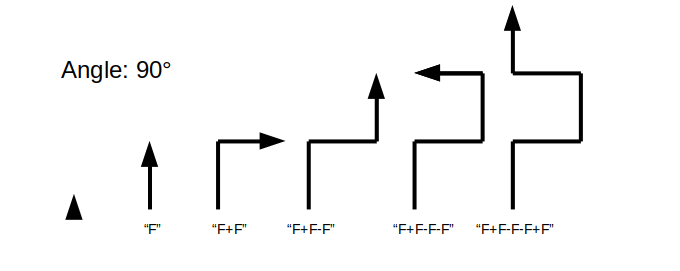
\includegraphics[scale=0.5]{Diagrams/basic_turtle.png}
		\caption{Diagram showing a turtle interpreting simple L-system string.}
	}
\end{figure}
\FloatBarrier

\section{Branching Filaments}

In the previous section there are two turtle commands in particular which were not covered. These are the square brackets "[", "]". The square bracket characters instruct the turtle object to save its position and current angle for use later on. This allows the turtle to jump back to a previous point facing the same direction as it was before, It could then branch in a different direction.\\
\\
A way to keep track of these saved locations is in the form of a stack structure. Each time the "[" is called the current position and direction of the turtle is saved to the top of the stack. Conversely when the "]" is called we restore the turtles position back to whatever position and direction is stored on the top of the stack structure. \\
\\
An example of this can be shown below in figure 2.2.\\

\begin{figure}[htbp]
	{\centering
		\vspace{7px}
		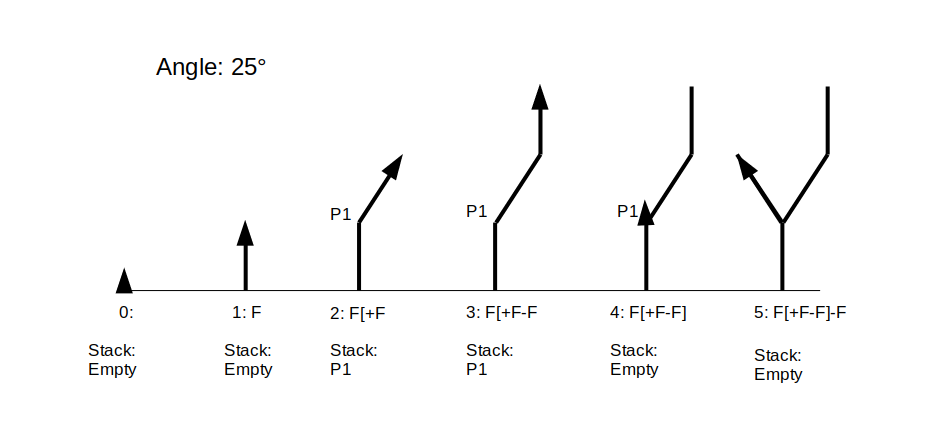
\includegraphics[scale=0.5]{Diagrams/branching_turtle.png}
		\caption{Diagram showing a turtle interpreting an L-system incorporating branching.}
	}
\end{figure}
\FloatBarrier


\section{Basic 2D L-systems} 

There are a number of fractal geometry that have become well known particularly with regards to how they can seemingly imitate nature \cite{mandelbrot1982fractal}. Particularly with the geometry such as the Koch snowflake which can be represented using the following L-system.

\begin{figure}[htbp]
	\raggedright
	\textbf{\underline{Koch Curve:}} \\
	\textbf{Alphabet:} F \\
	\textbf{Constants:} +, - \\
	\textbf{Axiom:} F \\
	\textbf{Angle:} 90$^\circ$ \\
	\textbf{Rules:} \\
	F $\rightarrow$ F+F--F+F\\
	{\centering
		\vspace{7px}
		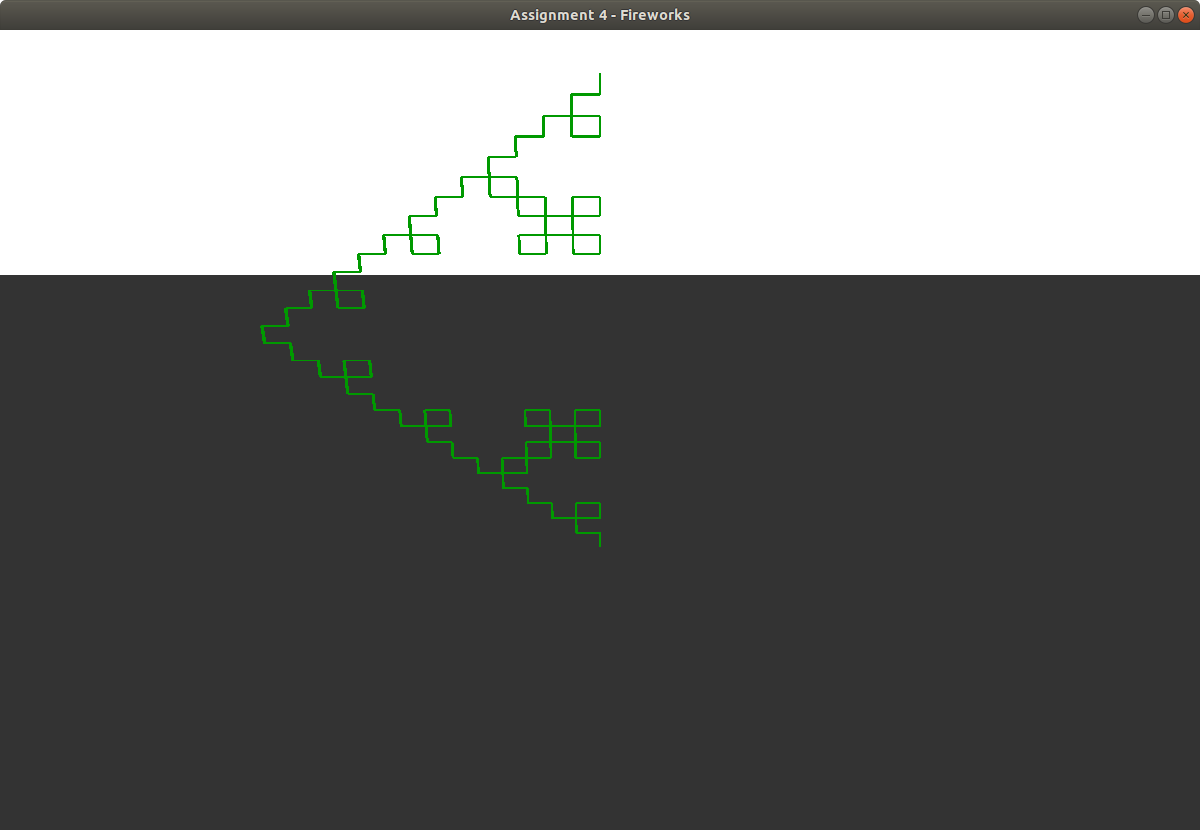
\includegraphics[scale=0.8]{KochCurve/KochCurve04.png}
		\caption{Koch Curve.}
	}
\end{figure}
\begin{figure}[htbp]
	\raggedright
	\textbf{\underline{Sierpinski Triangle:}} \\
	\textbf{Alphabet:} A, B \\
	\textbf{Constants:} +, - \\
	\textbf{Axiom:} A \\
	\textbf{Angle:} 60$^\circ$ \\
	\textbf{Rules:} \\
	A $\rightarrow$  B-A-B \\
	B $\rightarrow$ A+B+A\\
	{\centering
		\vspace{7px}
		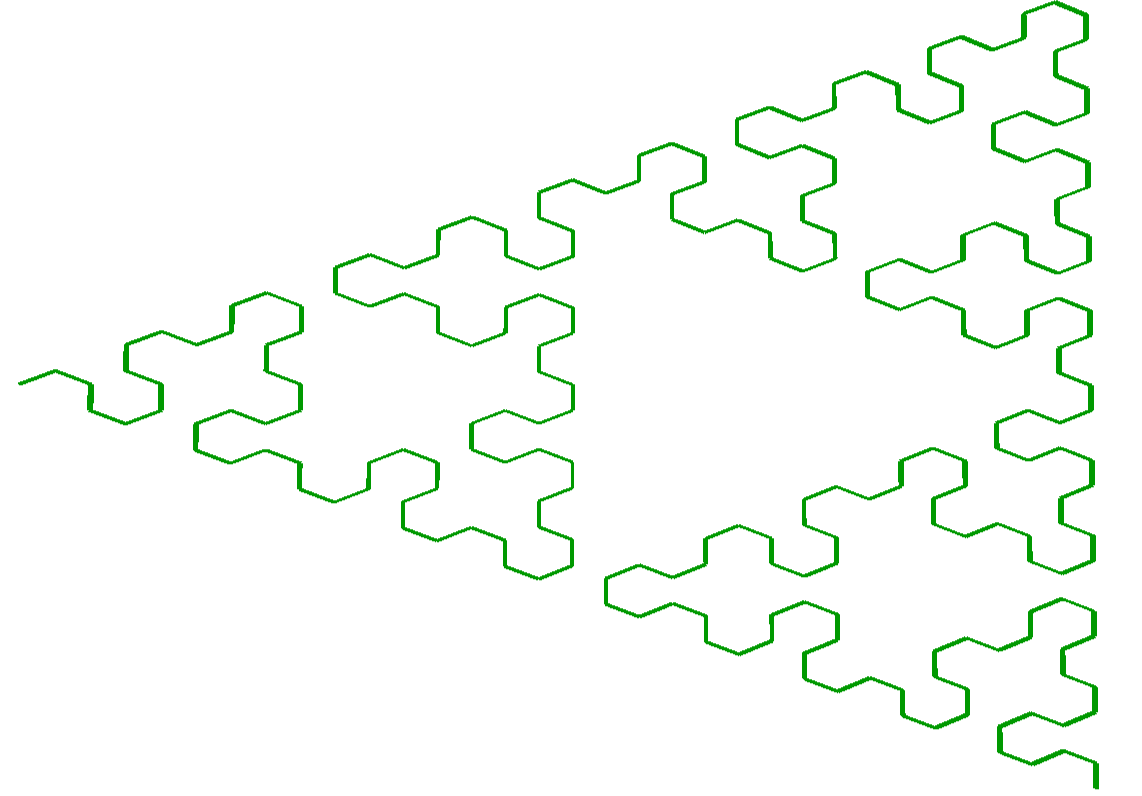
\includegraphics[scale=0.17]{SierpinskiTriangle/SierpinskiTriangle06.png}
		\caption{Sierpinski Triangle.}
	}
\end{figure}
\begin{figure}[htbp]
	\raggedright
	\textbf{\underline{Dragon Curve:}} \\
	\textbf{Alphabet:} F, X, Y \\
	\textbf{Constants:} +, - \\
	\textbf{Axiom:} FX \\
	\textbf{Angle:} 90$^\circ$ \\
	\textbf{Rules:} \\
	X $\rightarrow$ X+YF+ \\
	Y $\rightarrow$ -FX-Y\\
	{\centering
		\vspace{7px}
		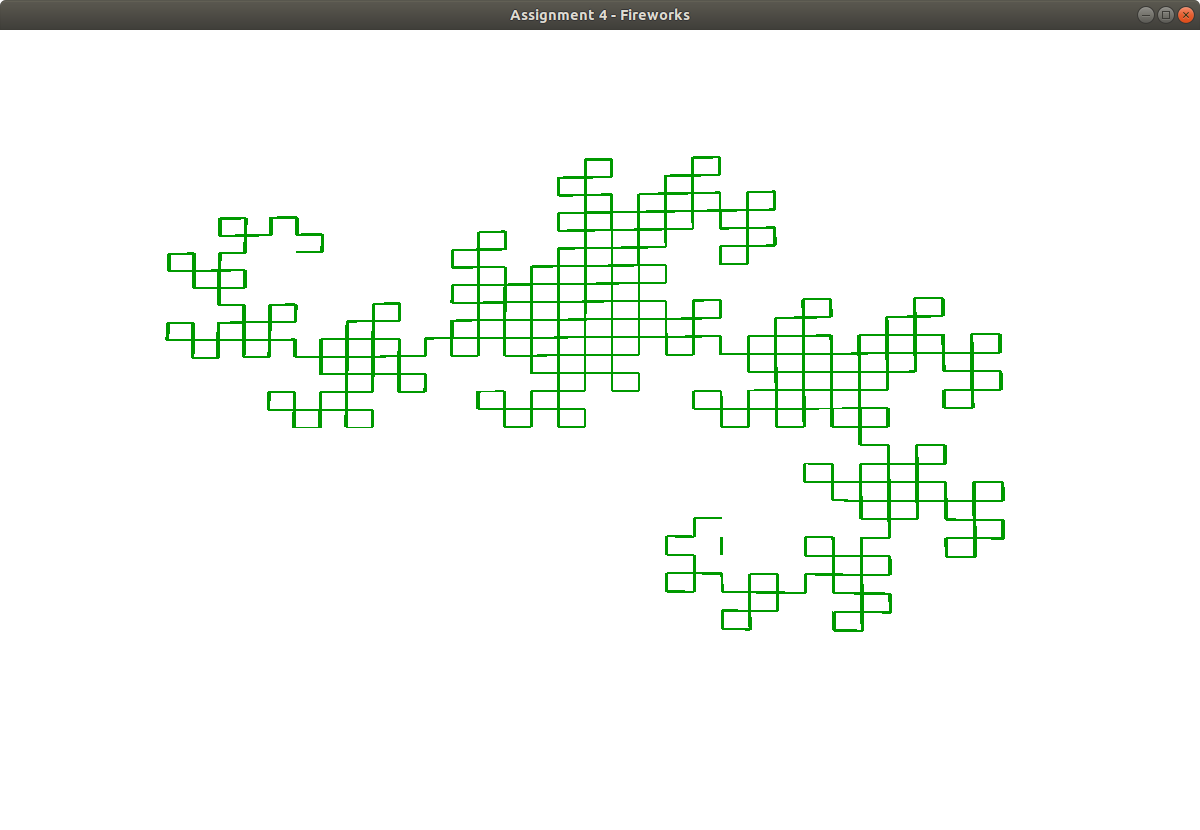
\includegraphics[scale=0.17]{DragonCurve/DragonCurve10.png}
		\caption{Dragon Curve.}
	}
\end{figure}
\begin{figure}[htbp]
	\raggedright
	\textbf{\underline{Fractal Plant:}} \\
	\textbf{Alphabet:} X, F\\
	\textbf{Constants:} +, -, [, ] \\
	\textbf{Axiom:} X \\
	\textbf{Angle:} 25$^\circ$ \\
	\textbf{Rules:} \\
	X $\rightarrow$ F-[[X]+X]+F[+FX]-X\\
	F $\rightarrow$ FF \\
	{\centering
		\vspace{7px}
		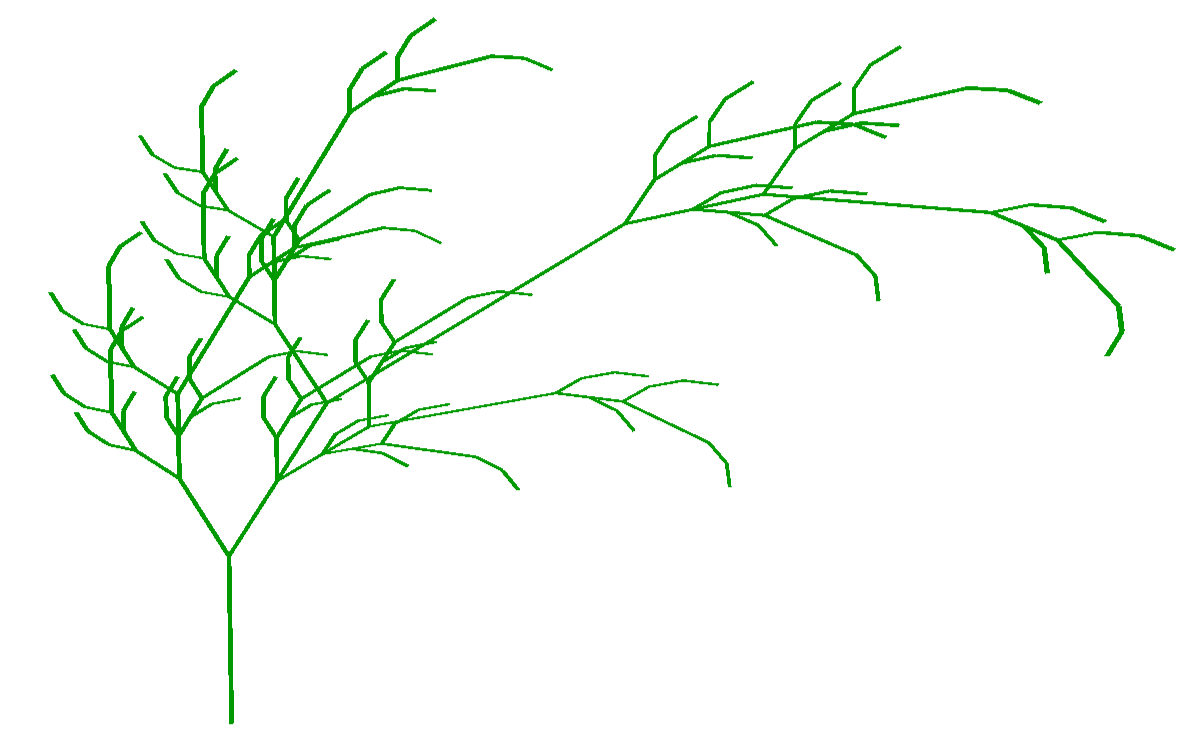
\includegraphics[scale=0.15]{FractalPlant/FractalPlant05.png}
		\caption{Fractal Plant.}
	}
\end{figure}
\begin{figure}[htbp]
	\raggedright
	\textbf{\underline{Fractal Bush:}} \\
	\textbf{Alphabet:} F\\
	\textbf{Constants:} +, -, [, ] \\
	\textbf{Axiom:} F \\
	\textbf{Angle:} 25$^\circ$ \\
	\textbf{Rules:} \\
	F $\rightarrow$ FF+[+F-F-F]-[-F+F+F]\\
	{\centering
		\vspace{7px}
		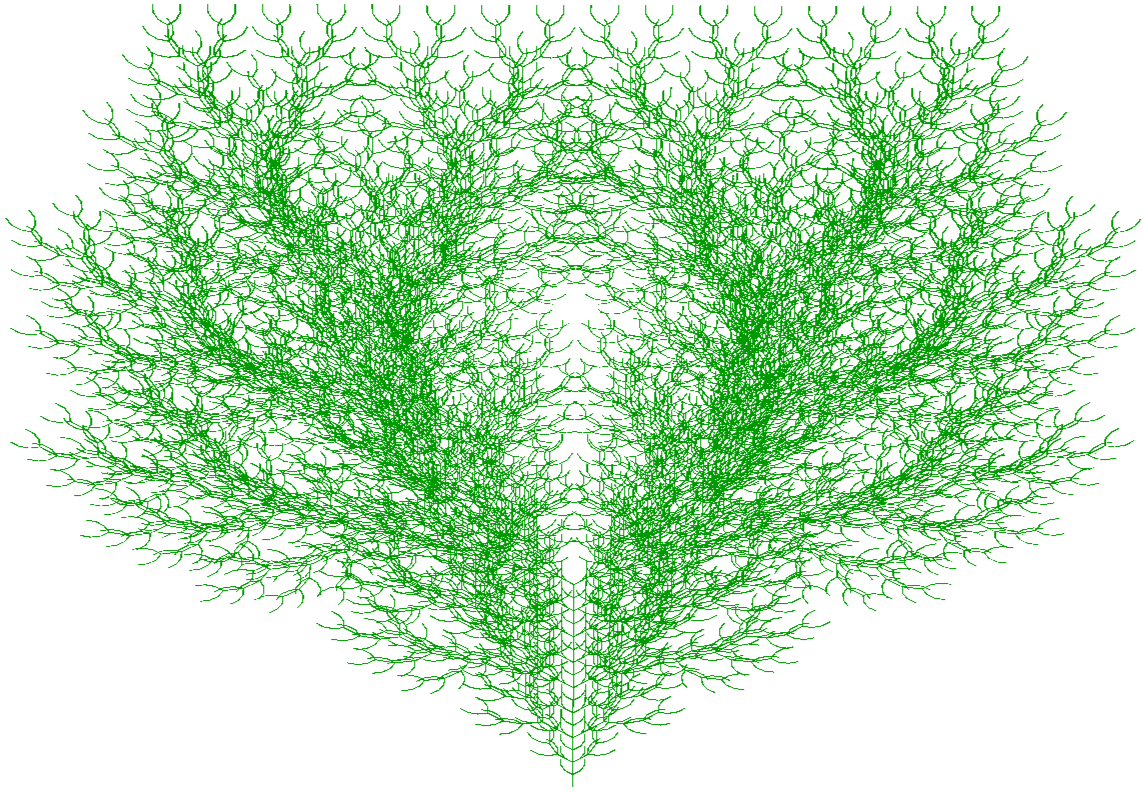
\includegraphics[scale=0.15]{FractalBush/FractalBush06.png}
		\caption{Fractal Bush.}
	}
\end{figure}

\FloatBarrier
\newpage

\section{The Use of L-systems in 3D applications}

L-systems have been talked about and researched since its inception in 1968 by Aristid Lindenmayer. Over the years it's usefulness in modelling different types of plant life has been very clear, however its presence has been quite absent from any mainstream game engines for the most part, these engines relying either on digital artists skill to develop individual plants or on 3rd party software such as SpeedTree. These types of software use a multitude of different techniques however their methods are heavily rooted in Lindenmayer Systems. 

\newpage

\section{Parametric L-system}

With simplistic L-systems like the algae representation above, there are a number of details that are skipped over when making this simplistic representation. (talk about the representation for both parameterized and non parameterised Algae systems). When it comes to representing trees as L-systems a simplistic approach would be to just assume that the width and length of each branch section is constant and will not vary depending on where in the tree it is. We can also assume that the angles at which a branch may split is also constant, say 25 degrees. 
The resulting representation of this L-system is a tree like structure, however it is not a very accurate representation of a real tree in nature. \\
In order to more accurately model trees we need to take into account the branch width, height, branching angles. There are two different approaches to solving this added complexity. One would be to increase the complexity of the L-system grammar and the other would be to increase the complexity of the interpretation of the L-system. \\
For instance defining an complex L-system grammar with a less complex interpreting system can give a huge amount of flexibility to define parameters that can accurately define exactly how the L-system should be interpreted, and because the complexity is with the L-system rewriting you also have the control of being able to change the L-system rules. \\
\\ 
A parametric l-system be represented as the following: \\
\\
\hspace*{3cm} n = 8\\
\\
\hspace*{3cm} \#define R 1.456\\
\hspace*{3cm} \#define r1 85\\
\hspace*{3cm} \#define wr 0.707\\
\\
\hspace*{3cm} w : A(5)\\
\\
\hspace*{3cm} p1 : A(w) : * : F(1)!(w)[/(r1)A(w*wr)][$\backslash$(r1)A(w*wr)]\\
\hspace*{3cm} p2 : F(s) : * : F(s*R)\\
\\
The above l-system gives the resulting representation shown below in figure 3.8. 

\begin{figure}[htbp]
	{\centering
		\vspace{7px}
		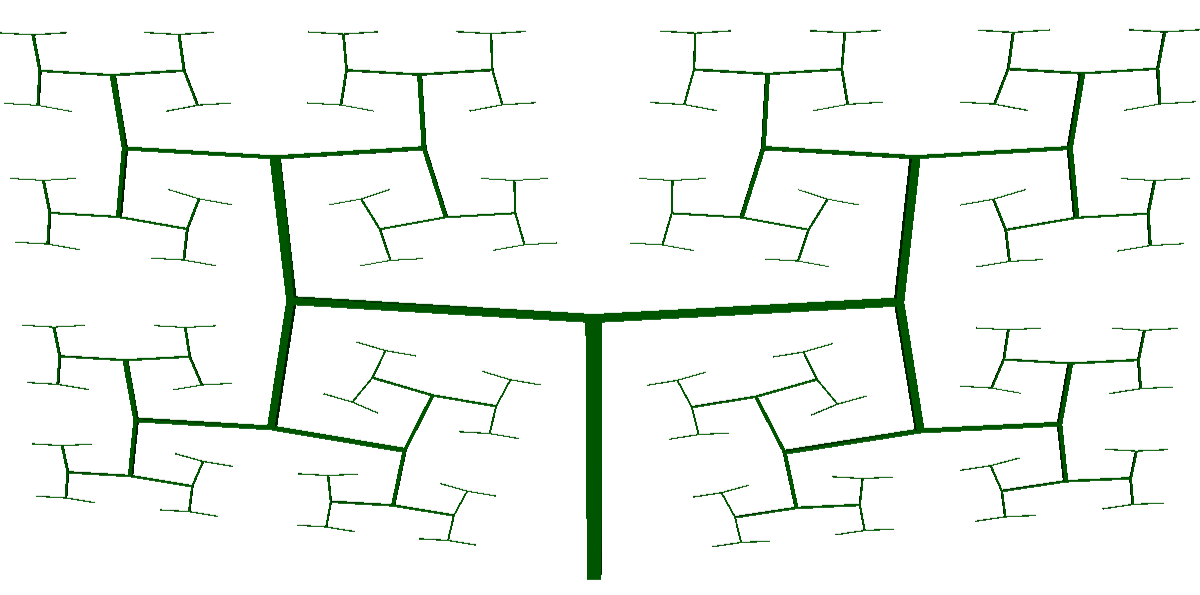
\includegraphics[scale=0.20]{ParametricLsystem/branchingPattern.png}
		\caption{3D Parametric L-system.}
	}
\end{figure}

Similarly to the 2D L-system in section \ref{Simple DOL-systems}, n refers to the number of iterations that we would like to rewrite the L-system. w refers to the Axiom string, the \#define R 1.456 states that there is a constant number that will be used somewhere in the production rules, with the name R and the value 1.456. P1, P2 refer to the production rules. The 3D L-system introduces the concept of a module.\\
A module is an instruction or variable which has zero or more parameters. The Axiom A(5) is a module with one parameter which is the number 5. A parameter can either be a number, variable or even an expression of variables and numbers. For instance A(a + 1, a * b) is a valid module A with two parameters a + 1 and a * b, where a and b are variables, however this is only a valid module if the value of a and b can be determined. Each module is treated as a single instruction, it will either be overwritten when matched with a production rule or the expression of each parameter is evaluated and is left unchaged for use when interpretted.\\
Each production rule is made up of four parts the name, the predecessor module, the condition and the successor modules, each part is separated by a colon. Therefor the predecessor for p1 is A(w), the condition is a '*' which means that in this case there are no conditions, and the successor is F(1)!(w)[/(r1)A(w*wr)][$\backslash$(r1)A(w*wr)]\\
\\
Initially we iterate through the Axiom modules and compare them to the production rule. A match is determined if they meet three criteria.\\
\\
$\bullet$ The name of the axiom module matches the name of the production predecessor. \\
$\bullet$ The number of parameters for the axiom module is the same as the number of parameters for the production predecessor. \\
$\bullet$ The condition of the production evaluates to true. If there is no condition then the result is true by default.\\
\\


\section{Formalising Parametric L-system Grammar}

With the grammar that has now been defined, we are now able to represent complex three dimensional tree structures in the form of a L-system rule set. In a computing sense this rule set can be seen as a type of program. In the program we define the number of generations we would like to generate, the starting point (Axiom) some constant varables (\#define) and the production rules. \\

\textless generations\textgreater~ ::= "\#n" "=" \textless float\textgreater~ ";" \\
\\
\textless definition\textgreater~ ::=  "\#define" \textless variable\textgreater~ \textless float\textgreater~ ";" \\
\\
\textless axiom\textgreater~ ::=  "\#w" ":" \textless moduleAx\textgreater~ ";" \\
\textless moduleAx\textgreater~  ::= \textless variable\textgreater~ $|$ "$+$" $|$ "$-$" $|$ "/" $|$ "$\backslash$" $|$ "$\hat{}$" $|$ "$\&$" $|$ "!" 

\hspace{1cm} \textless variable\textgreater~ "("  \textless paramAx\textgreater~ \textless paramListAx\textgreater~ ")"

\hspace{1cm} $|$ "$+$" "("  \textless paramAx\textgreater~ \textless paramListAx\textgreater~ ")" 

\hspace{1cm} $|$ "$-$""("  \textless paramAx\textgreater~ \textless paramListAx\textgreater~ ")" 

\hspace{1cm} $|$ "/""("  \textless paramAx\textgreater~ \textless paramListAx\textgreater~ ")" 

\hspace{1cm} $|$ "$\backslash$""("  \textless paramAx\textgreater~ \textless paramListAx\textgreater~ ")" 

\hspace{1cm} $|$ "$\hat{}$ " "("  \textless paramAx\textgreater~ \textless paramListAx\textgreater~ ")" 

\hspace{1cm} $|$ "$\&$" "("  \textless paramAx\textgreater~ \textless paramListAx\textgreater~ ")" \\
\textless paramAxList\textgreater~ ::=  $\in$ $|$ ":" \textless paramAx\textgreater~ \textless paramAxList\textgreater~ \\
\textless paramAx\textgreater~ ::= \textless float\textgreater~ \\
\\
\textless production\textgreater~ ::=  "\#" \textless variable\textgreater~  ":" \textless module\textgreater~ ":" \textless condition\textgreater~  ":" \textless successor\textgreater~ ";"\\
\textless module\textgreater~ ::=  \textless variable\textgreater~ $|$ "$+$" $|$ "$-$" $|$ "/" $|$ "$\backslash$" $|$ "$\hat{}$" $|$ "$\&$" $|$ "!" 

\hspace{1cm} \textless variable\textgreater~ "("  \textless param\textgreater~ \textless paramList\textgreater~ ")"

\hspace{1cm} $|$ "$+$" "("  \textless param\textgreater~ \textless paramList\textgreater~ ")" 

\hspace{1cm} $|$ "$-$""("  \textless param\textgreater~ \textless paramList\textgreater~ ")" 

\hspace{1cm} $|$ "/""("  \textless param\textgreater~ \textless paramList\textgreater~ ")" 

\hspace{1cm} $|$ "$\backslash$""("  \textless param\textgreater~ \textless paramList\textgreater~ ")" 

\hspace{1cm} $|$ "$\hat{}$ " "("  \textless param\textgreater~ \textless paramList\textgreater~ ")" 

\hspace{1cm} $|$ "$\&$" "("  \textless param\textgreater~ \textless paramList\textgreater~ ")" \\
\textless paramList\textgreater~ ::=  $\in$ $|$ ":" \textless param\textgreater~ \textless paramList\textgreater~ \\
\textless param\textgreater~ ::= \textless float\textgreater~ \\
\\
\textless expression\textgreater~ ::=  \textless expression\textgreater~ \textless symbol\textgreater~ \textless expression\textgreater~ $|$ 
\\
\textless float\textgreater~ ::= [0-9]+.[0-9]+ \\
\textless variable\textgreater~ ::= [a-zA-Z\_][a-zA-Z0-9\_]* \\



